\chapter{Analysis}


Since .NET is a managed environment, the documentation generators can be classified into 2 categories depending on what their input is:

\begin{itemize}
    \item Source code
    \item Intermediate language
\end{itemize}

The generators that use source code as an input, for instance, Doxygen, may seem straightforward; however, they typically have the following disadvantages:
\begin{enumerate}
    \item Language coupling -- The generator is coupled to the given language. 
    Adding support for a new language requires the creation of a new parser for it, which is a complex task.
    \item Complexity -- In general, these generators are quite hard to develop because an actual parsing of the language is needed in order to obtain the type and member definitions.
\end{enumerate}

Generators that use intermediate code as their input, such as SHFB, are typically easier to develop and also don't suffer from the issues mentioned earlier.
These generators aren't limited to a single language; in the case of .NET, a single generator can handle e.g. C\#, F\#, and Visual Basic programs. 
One downside is the need for program compilation, so the project must be built before the documentation is generated.
However, this is not a limiting factor for us.

(TODO: mozna nejak vice rozepsat, ale zadne dalsi vylozene minus me nenapada)

Using this information, we can refine our primary goal -- to develop a reference
documentation generator for .NET that uses intermediate code as its input.

\section{Compilation process in .NET}

Since our generator will use the assembly, we'll describe the compilation process in .NET a little bit more in detail.

As stated in the .NET documentation~\cite{dotnet_execution_model} and illustrated in Figure~\ref{fig:net_compilation}, 
the compilation translates the source code of the program into the common intermediate language (CIL), which is a CPU-independent set of instructions that can be efficiently converted to native code. 
CIL includes instructions for loading, storing, initializing, and calling methods on objects, as well as instructions for arithmetic and logical operations, control flow, and other operations.

Along CIL, the compiler also produces metadata, which describes the types in the code, including the definition of each type, the signatures of its members, and other data that the runtime uses at execution time, according to~\cite{dotnet_execution_model}.
The CIL and metadata are contained in a .NET assembly, which is typically a dynamic link library (\texttt{.dll}) or executable (\texttt{.exe}) file.

Note that the only part we need as developers of the documentation generator is the metadata.
We don't need to use the CIL, because we won't execute any code of the program.

\hfill

(asi vyhodit, protoze to nepotrebujeme + upravit obrazek)

At runtime, CIL is converted to CPU-specific code on demand, by a just-in-time (JIT) compiler. 
There is a JIT compiler for each computer architecture that .NET supports and therefore, the same CIL can be JIT-compiled and run on any supported architecture.

\begin{figure}
\centering
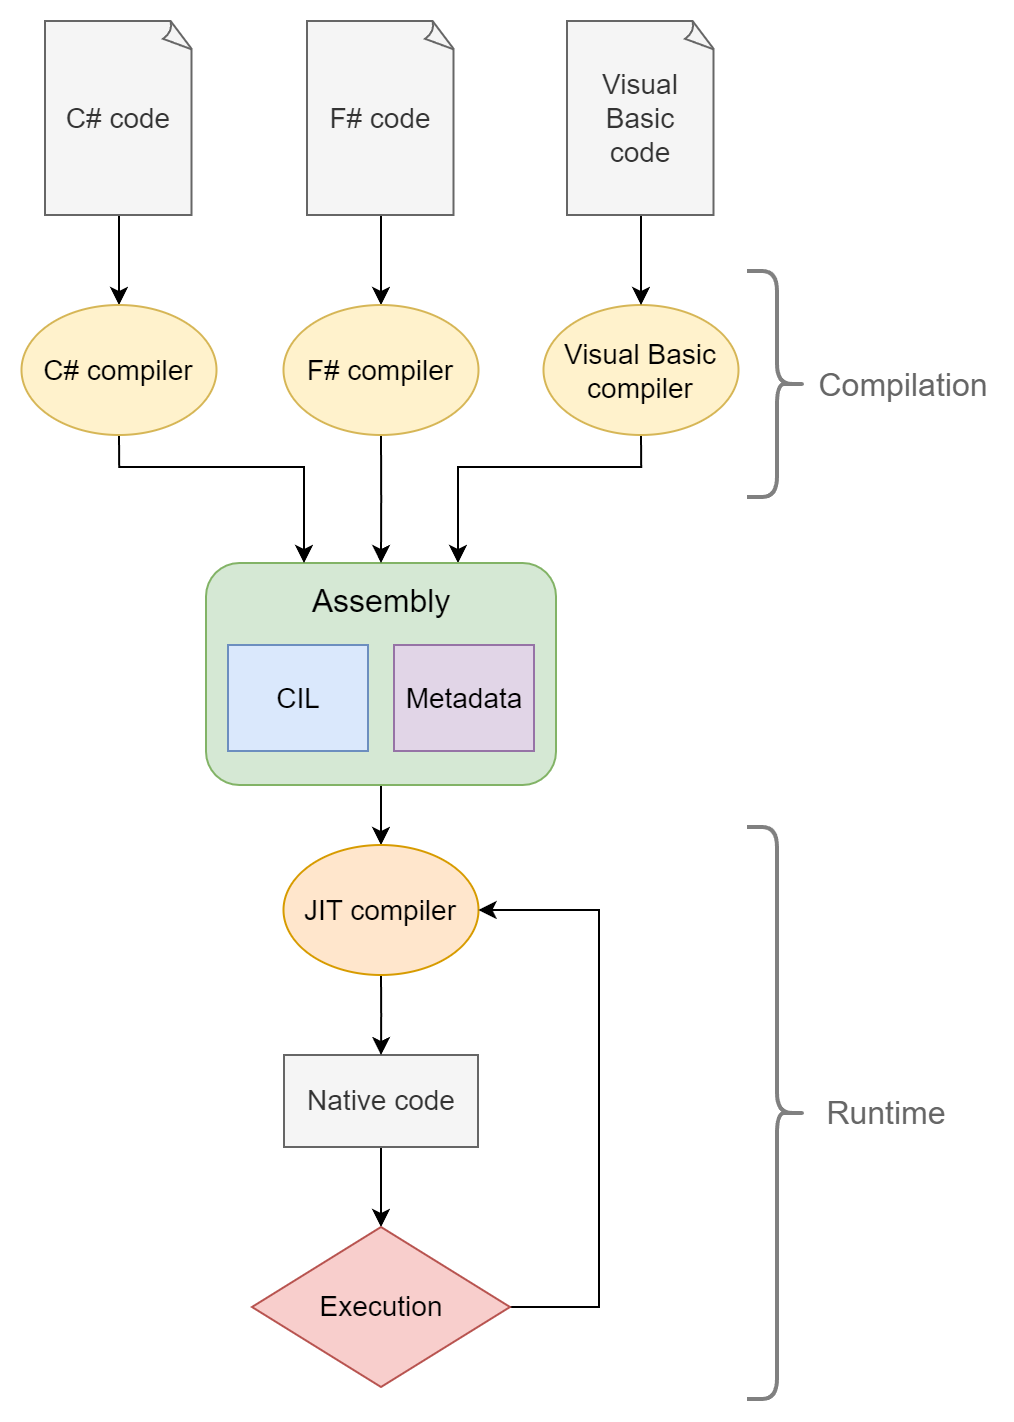
\includegraphics[width=1\linewidth]{img/compilation.png}
\caption{Execution of a .NET program}
\label{fig:net_compilation}
\end{figure}

\section{Reflection}
(TODO: mozna prejmenovat kapitolu na "Extracting the data from assembly" ?)

Now, we know what the assembly is and how it is created, yet we still haven't mentioned how to extract the type and member information from it.
This is done using reflection, which in general refers to the ability of a program to inspect or modify other code (or itself).

First of all, it's necessary to load the assembly that is going to be documented, which is done using the \texttt{Assembly.Load} method.
Then, we can obtain all the declared types, represented as \texttt{System.Type} instances, by calling the \texttt{GetTypes} method of the loaded assembly.

The \texttt{System.Type} class represents any type: class, interface, array type, value type, enumeration, delegate, or type parameter.
Using its members, we can discover any data concerning the type (such as whether it is abstract, sealed, etc.), as described in .NET documentation~\cite{dotnet_reflection}.

Methods of a type can be obtained by calling the \texttt{GetMethods} method (there are analogous methods for the other members).
The type members are represented by the following classes (each representing
the corresponding member and providing descriptive information about it, as stated in~\cite{dotnet_reflection}): (TODO: ma zde byt citace?)

\begin{itemize}
    \item \texttt{ConstructorInfo}
    \item \texttt{FieldInfo}
    \item \texttt{EventInfo}
    \item \texttt{MethodInfo}
    \item \texttt{PropertyInfo}
\end{itemize}

There is also the \texttt{ParameterInfo} class, which provides information about a method (or constructor) parameter. 

Example~\ref{lst:ex-reflection} shows a code snippet that prints the return type and name of all methods contained in the type \texttt{Person}.
Notice that something similar, obviously much more complex, will be performed by the documentation generator.
The snippet may thus serve as a good starting point for the type and member data extraction.

\begin{listing}
\begin{lstlisting}
Type personType = typeof(Person);

foreach (MethodInfo method in personType.GetMethods())
{
    Console.WriteLine(
        $"{method.ReturnType.Name} {method.Name}");
}
\end{lstlisting}
\caption{Code that inspects type methods using reflection}
\label{lst:ex-reflection}
\end{listing}

\section{XML documentation comments}

(TODO: mozna prejmenovat kapitolu na "Extracting documentation comments" ?)

Note that extraction of the documentation comments wasn't mentioned in the previous chapter.
That's because the comments aren't present in the assembly, and therefore we can't use reflection in any way to access them.

Firstly, it's worth noting that the vast majority of .NET languages use structured XML comments, well known from C\#, to document types and their members.
Example~\ref{lst:ex-xml-doc-method} shows a method with XML documentation; 
notice that both parameters and the return value are documented as well (using the \texttt{param} and \texttt{returns} tag, respectively).

Previously, we mentioned that the documentation comments aren't part of the assembly.
Instead, when compiling to CIL, the compiler can optionally create an XML file containing the documentation of the declared types and their members.
This is typically done by setting the \texttt{GenerateDocumentationFile} or \texttt{DocumentationFile} 
option, as mentioned in the MSBuild documentation~\cite{msbuild_docs}.

Example~\ref{lst:ex-xml-output} shows the resulting XML file containing the method documentation shown in Example~\ref{lst:ex-xml-doc-method}.
As we can see, the comments are stored inside the \texttt{member} element that contains a \texttt{name} attribute, which uniquely identifies the corresponding type or member.

\begin{listing}
\begin{lstlisting}
/// <summary>
/// Calculates the area of a rectangle given its width
/// and height.
/// </summary>
/// <param name="width">Width of the rectangle.</param>
/// <param name="height">Height of the rectangle.</param>
/// <returns>The area of the rectangle.</returns>
public static double CalculateRectangleArea(
    double width, double height)
{
    return width * height;
}
\end{lstlisting}
\caption{Example of an XML-documented method}
\label{lst:ex-xml-doc-method}
\end{listing}

\begin{listing}
\begin{lstlisting}
<?xml version="1.0"?>
<doc>
    <assembly>
        <name>MyApp</name>
    </assembly>
    <members>
        <member name="M:MyApp.MyClass.CalculateRectangleArea
                            (System.Double,System.Double)">
            <summary>
                Calculates the area of a rectangle given 
                its width and height.
            </summary>
            <param name="width">
                Width of the rectangle.
            </param>
            <param name="height">
                Height of the rectangle.
            </param>
            <returns>
                The area of the rectangle.
            </returns>
        </member>
        ...
    </members>
</doc>
\end{lstlisting}
\caption{Example of the resulting XML documentation file}
\label{lst:ex-xml-output}
\end{listing}

The extraction of the documentation comments will be another task performed by our generator, along with the reflection usage.
To outline the process, we first need to parse the XML file. Then we can assign individual comments to the corresponding types or type members, identified by the \texttt{name} attribute.

\section{XML documentation tags}

Interestingly, the set of XML documentation tags isn't explicitly declared. 
Instead, there's a set of recommended tags described in the official documentation.
As a consequence, any XML tag is valid and can be used in the documentation 
(although in this case, it may not be correctly interpreted in the output).

The recommended tags used in all .NET languages are the following:

\subsection{Summary}
The \texttt{summary} tag is the most commonly used documentation tag and provides a description of a type or member. 
It can be applied to any type or member.

\subsection{Remarks}
The \texttt{remarks} can also document any type or member. 
Its purpose is to document any additional information not covered by the \texttt{summary} tag.

\subsection{Param}
The \texttt{param} tag documents a parameter, which is identified by the \texttt{name} attribute.

\subsection{Returns}
The \texttt{returns} tags provides documentation for a method's return value.

\subsection{Typeparam}

\subsection{Exception}

\subsection{Value}

\subsection{Paramref}

\subsection{Typeparamref}

\subsection{See}

\subsection{Seealso}

\subsection{Para}

\subsection{C}

\subsection{Code}

\subsection{Example}

\subsection{List}

\subsection{Item}

\subsection{Inheritdoc}

\subsection{Include}

\section{Existing Technologies}

\subsection{Doxygen}

Doxygen is a well-established documentation generator that supports many languages, including C++, C\#, Java, PHP, and Python.
It is a typical example of a generator parsing source code; 
interestingly, there is a shared parser for all languages implemented using \texttt{flex}.~\cite{doxygen_docs} 

Doxygen is highly configurable, offering more than 300 various options.

TODO: rozepsat options? Nebo staci jen link?

The configuration is stored as a collection of key-value pairs in a configuration file, typically called \texttt{Doxyfile}.
The downside of the extensive option support is the complexity of the configuration file,
which has by default over 2000 lines (most of the content consists of the individual option documentations, though).

The documentation is built by running \texttt{Doxygen} from the command line.
In addition to HTML, there are multiple output formats available, such as LaTeX and XML.
Doxygen can also be used for user documentation, as it allows us to include custom static pages from the provided files in \texttt{.dox}, \texttt{.txt}, or \texttt{.md} format.~\cite{doxygen_docs}

By default, the documentation may be created in a light or dark mode; however, Doxygen supports further customization at various levels.
It is possible to provide a custom stylesheet, page fragment, or the whole layout.

An example reference documentation generated by Doxygen is shown in Figures \ref{fig:doxygen1} and \ref{fig:doxygen2}. Notice that the default UI is unfortunately quite old-school.

\begin{figure}
\centering
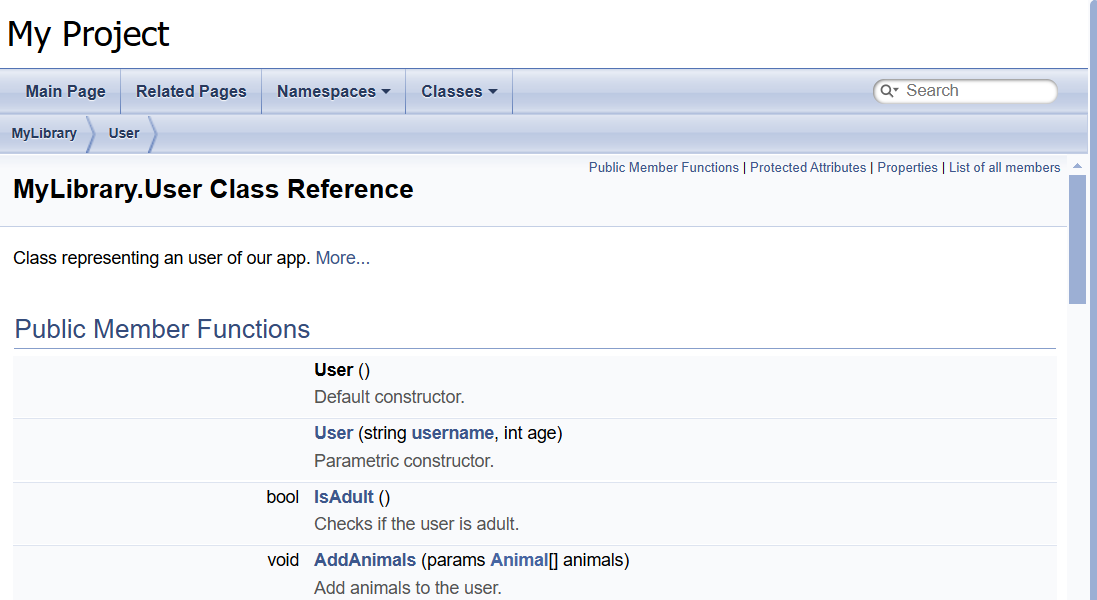
\includegraphics[width=1\linewidth]{img/doxygen1.png}
\caption{Documentation generated by Doxygen -- type detail}
\label{fig:doxygen1}
\end{figure}

\begin{figure}
\centering
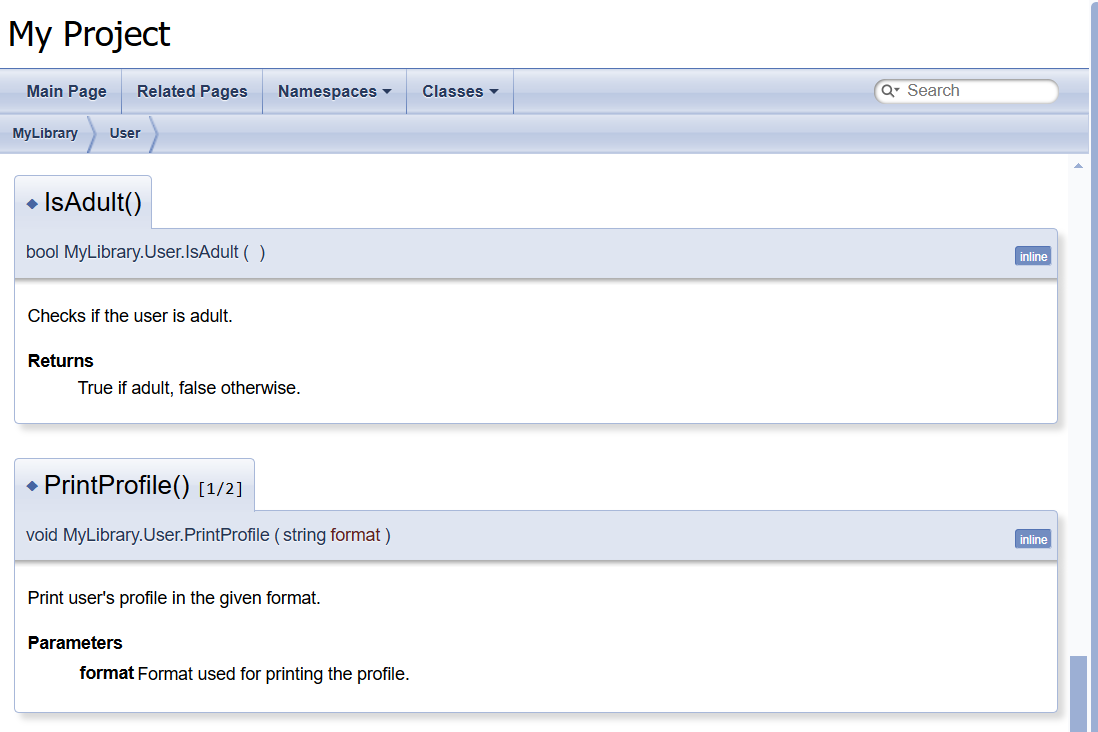
\includegraphics[width=1\linewidth]{img/doxygen2.png}
\caption{Documentation generated by Doxygen -- members detail}
\label{fig:doxygen2}
\end{figure}

\subsection{DocFX}


DocFX is a popular reference documentation generator, that can be also used as a static site generator. 

It can process both compiled assemblies and source code.

Configuration in docfx.json

installed as a .NET tool.

Several templates available by default.

Custom templates: Using HTML and CSS

\subsection{Sandcastle Help File Builder}

Sandcastle Help File Builder (SHFB) is another documentation generator for .NET.
It uses reflection to extract the data from the assembly.

The configuration is stored in a standard MSBuild-format project file.
This means that the documentation can be built using \texttt{dotnet build} or \texttt{msbuild} command.

SHFB supports several custom documentation tags, for instance \texttt{threadsafety} tag denoting the thread safety of the member.

There are several output formats available: HTML, Markdown, and Open XML document.
The default HTML template has a separate page for each member.

TODO: customization

The default UI is shown in Figure \ref{fig:shfb1} -- type detail and Figure \ref{fig:shfb2} -- method detail.

The major disadvantage of SHFB, is that it requires .NET framework, therefore it cannot be run outside Windows.

\begin{figure}
\centering
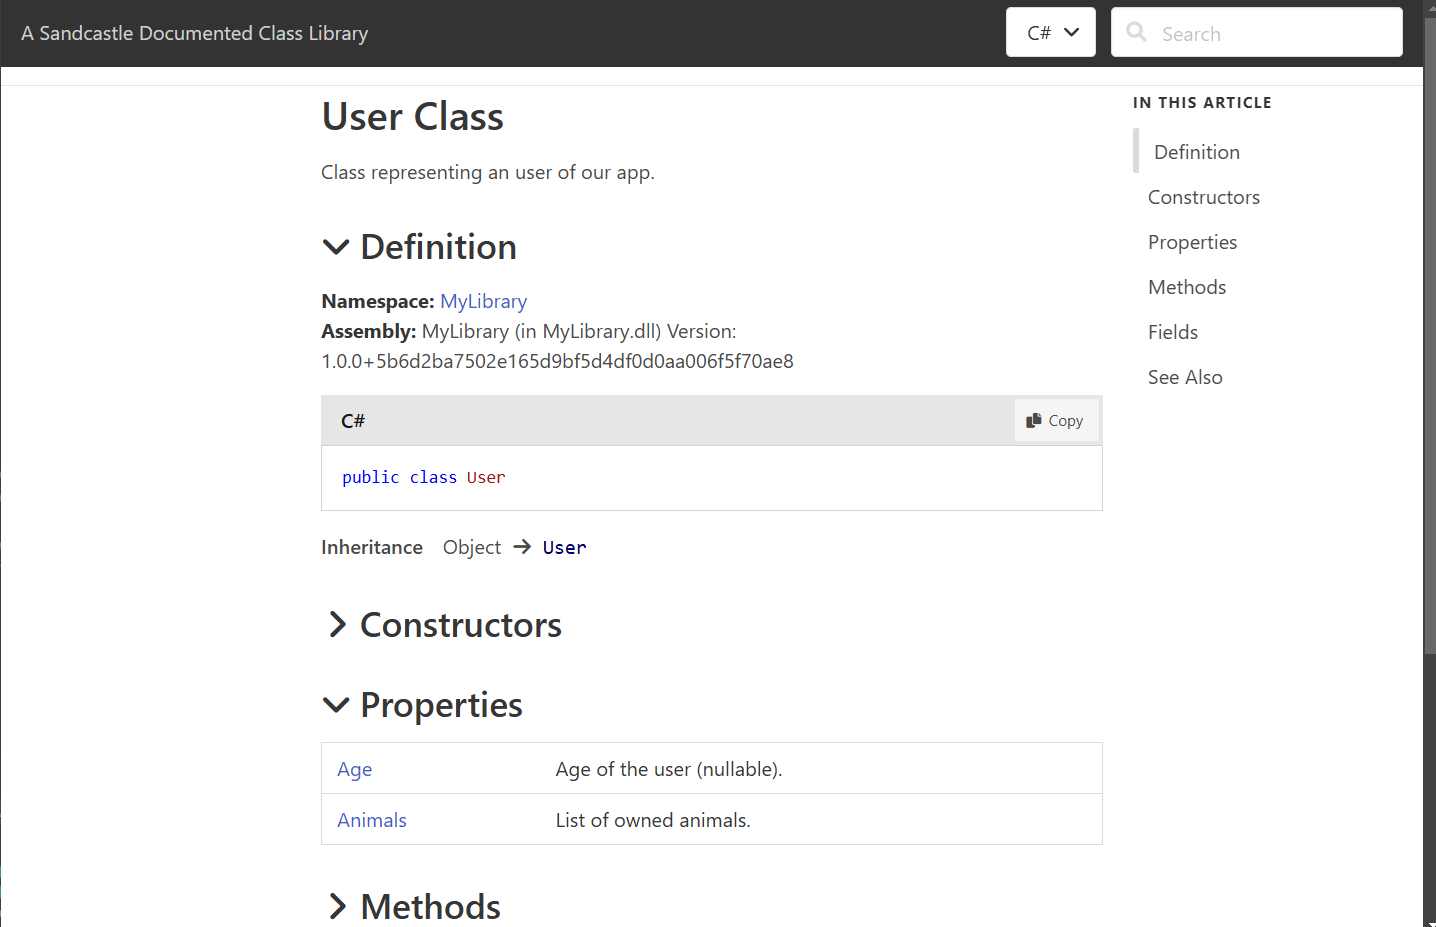
\includegraphics[width=1\linewidth]{img/sandcastle1.png}
\caption{Documentation generated by SHFB -- type detail}
\label{fig:shfb1}
\end{figure}

\begin{figure}
\centering
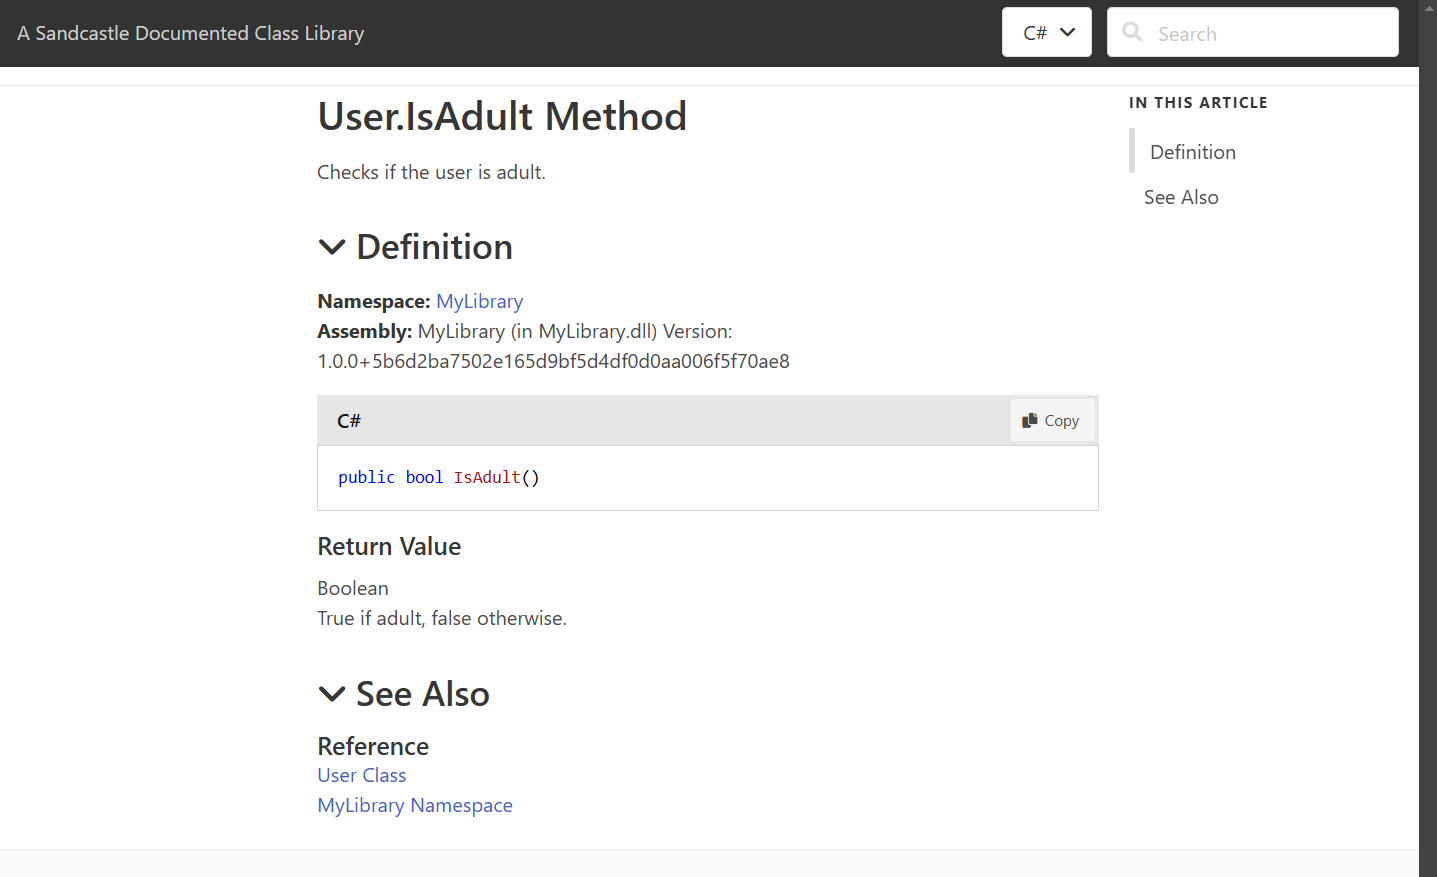
\includegraphics[width=1\linewidth]{img/sandcastle2.png}
\caption{Documentation generated by SHFB -- method detail}
\label{fig:shfb2}
\end{figure}

\subsection{JavaDoc}

Javadoc is a documentation generator for Java; furthermore, it is even part of the JDK.

The javadoc command parses the declarations and documentation comments in a set of Java source files and produces a corresponding set of HTML pages that describe (by default) the public and protected classes,

Can be run from command line.

Super easy to use - no configuration. 
However, configuration is possible using project file.

By default, it supports only HTML output, others can be achieved using (or writing own) extensions.

\subsection{Sphinx}

Sphinx is a documentation generator or a tool that translates a set of plain text source files into various output formats, automatically producing cross-references, indices, etc. That is, if you have a directory containing a bunch of reStructuredText or Markdown documents, Sphinx can generate a series of HTML files, a PDF file (via LaTeX), man pages and much more.

Sphinx focuses on documentation, in particular handwritten documentation, however, Sphinx can also be used to generate blogs, homepages and even books. Much of Sphinx’s power comes from the richness of its default plain-text markup format, reStructuredText, along with its significant extensibility capabilities.

Quite complex configration options, many files.

Originally for Python, but includes support for other languages such as JavaScript and C++.

Many built in themes, rtd is quite popular.

\section{Goals (or Requirements)}

\subsection{Separate Page for Each Type Containing Its Members}
TODO: nechat? pridat nejaky nakres?
\subsection{List of Namespaces and Types Contained}
\subsection{Cross-references support}

The parameter and return types should contain a link to their definition, if possible.
The same applies to the types and members referenced by \texttt{<see>} of \texttt{<seealso>} tags.

Support for the types declared in the same project is mandatory.
Optionally, we can also add support for standard library types.

\subsection{Search bar}
There should be a search bar at the top of the page, allowing the user to search for the types and members.

\subsection{Zero Configuration Build}
\subsection{Support for Selecting Just the Specified Assemblies}
\subsection{Support for Selecting Types/Elements with the Given Accessibility}
\subsection{Modern Looking UI}
\subsection{Support for Custom Templates}
\subsection{Multiplatform}
\subsection{Installation as a .NET Tool}
\subsection{Support for Documentation Versioning}
\subsection{Support for .NET Languages}

\section{Feature comparison}
Include a table that compares the application with the existing tools.
